\documentclass[10pt]{article}
\usepackage{preference}

\usepackage[dvipsnames]{xcolor}
\usepackage{listings}
\definecolor{codegreen}{rgb}{0,0.6,0}
\definecolor{codegray}{rgb}{0.5,0.5,0.5}
\definecolor{codepurple}{rgb}{0.58,0,0.82}
\definecolor{backcolour}{rgb}{0.95,0.95,0.92}

\lstdefinestyle{myStyle}{
    backgroundcolor=\color{backcolour},   
    commentstyle=\color{codegreen},
    keywordstyle=\color{magenta},
    numberstyle=\tiny\color{codegray},
    stringstyle=\color{codepurple},
    basicstyle=\ttfamily\footnotesize,
    breakatwhitespace=false,         
    breaklines=true,                 
    captionpos=b,                    
    keepspaces=true,                 
    numbers=left,                    
    numbersep=5pt,                  
    showspaces=false,                
    showstringspaces=false,
    showtabs=false,                  
    tabsize=2,
    extendedchars=\true
}

\lstset{style=myStyle}
\lstset{language=Python}

\begin{document}

\def\chap#1#2{\ \\ {\large\bf#1 \ | \ \tt\scshape#2} \par}

\vspace{-1cm}

{\bf
\ \\
\Large\centerline{\scshape Алгоритмы и структуры данных, лекции}
}\normalsize

\chapter{Паросочетания и потоки}

Мы начнём с паросочетаний и потоков.

\section{Паросочетания}
Паросочетание графа --- это набор его ребер, не имеющих общих вершин.

\subsection{Паросочетание в двудольном графе}
Паросочетания в двудольных графах ищутся гораздо проще, чем в произвольных.
Алгоритмы решают эту задачку понемногу. 
Берется маленькое (пустое) паросочетание и расширяется с помощью дополняющих цепочек.

Дополняющая цепочка --- это путь, который начинается и заканчивается в вершинах вне паросочетания, и ребра в нём чередуются (принадлежит - не принадлежит пар. сочетанию).
Из такой цепочки можно получить паросочетание большего размера (на 1).

Алгоритм начинает строить цепочки и удаляет дополняющие цепочки такой заменой.
\begin{theorem}
    В графе нет дополняющего пути тогда и только тогда, когда паросочетание максимально.
\end{theorem}
Это утверждение сформулировано для произвольных графов: для двудольных и не очень.
А в чём проблема? 
Проблема в поиске дополняющих путей.

В двудольном графе это делается просто. 
Это алгоритм Куна.

Двудольный граф можно хранить не как нормальный граф.
''Алгоритм КУНА. Это не связано с аниме никак!''
''Код, на самом деле, за пять копеек.''
Асимптотика: $O(nm)$.
% fn dfs(v):
% if mark[v]: return False;
% mark[v] = True

% for u \in G[v]:
%     if p[u] = \emptyset or dfs(p[u]):
%         p[u] = v
%         return True

% return False

% for v = 1..n
    % fill(mark, False)
    % dfs(v)

Алгоритм никогда не освобождает вершины --- если вершшина попала в пар. соч., она там останется, можно dfs из неё не запускать.
Чуть сложнее: если dfs однажда не нашел доп. пути из одной вершины, он никогда его не найдёт --- можно его не запускать.


Немного о полных сочетаниях.
\begin{theorem}
В двудольном графе $G_{n,n}$ существует полное паросочетание в том и только том случае, когда для любого подмножества $A$ вершин одной доли выполнено $|N(A)| \geqslant |A|$. 
\end{theorem}

Паросочетания позволяют решать кучу прикольных задач.

\subsection{Вершинное покрытие}
Вершинное покрытие в графе --- это набор вершин, таких, что никаие две вершины не лежат на одном ребре.
Это понятие двойственное понятию паросочетания.
Мы ищем минимальное по мощности вершинное покрытие. 
Это $NP$-полная задача в произвольном графе.
В двудольном, однако, всё очень мило.

Размер покрытия в графе всегда не превосходит размер вершинного покрытия: $M \leqslant S$.


\subsection{Парасочетание в недвудольном графе}

Так же понемногу будем искать дополняющие пути и достраивать наше паросочетание.

Как уже было доказано, $M$ --- max парсоч $\iff$ не.~~~~т дополняющих путей.

Как искать дополняющие пути? Может быть заюзать \texttt{dfs}?

\begin{lstlisting}[mathescape=true]
    dfs(v, state)
        ...
    for n
        if state:
            (u,v) $\in$ M
        else:
            (u,v) $\in$ M
        dfs(n, !state)
\end{lstlisting}


Но так нельзя!

На таком графе не сработает:

\begin{center}
    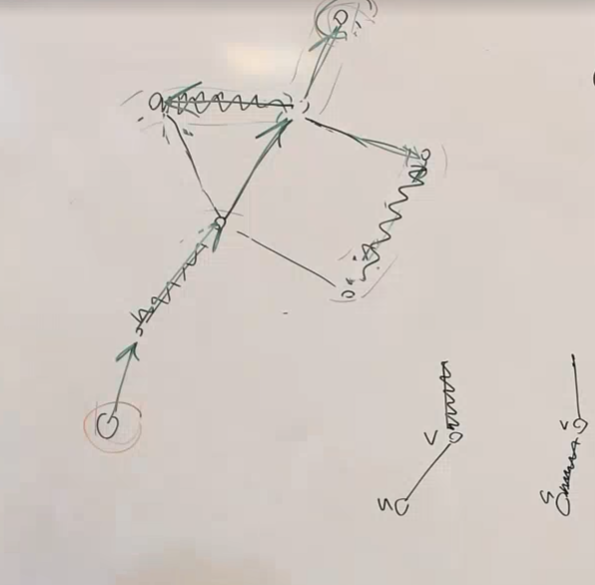
\includegraphics[scale=0.6]{img/parsoch_dfs_bad_usage}
\end{center}

Проблема в том, что в какую-то вершину мы можем прийти с неправильной четностью.

\textit{\textbf{Утверждение}}: если такого не случилось, то все будет ок.\\
Пусть есть стартовая вершина.
Назовем вершину сомнительной, если до нее есть четный и нечетный пути. \\
Если в графе нет сомнительных вершин, такой граф можно переделать в двудольный и легко в нем постить паросочетание.

\begin{center}
    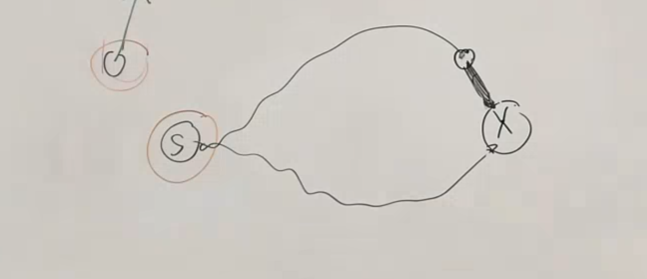
\includegraphics[scale=0.6]{img/parsoch_dfs_even_and_odd_paths}
\end{center}

Что делать?
Давайте запустим такой dfs.
Может быть три случая:
\begin{enumerate}
    \item Нашли дополняющий путь;
    \item Не нашли дополняющий путь и нет сомнительных вершин $\implies$ паросочетание макисмальное;
    \item Нашли сомнительную вершину.
\end{enumerate}

Если случилось третье, будем веселиться.
При помощи того же dfs-а найдем соцветие (blossom).
Внутри соцветия цикл нечетной длинны.

\begin{center}
    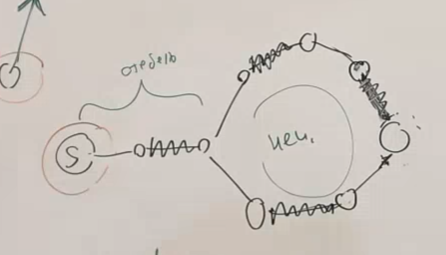
\includegraphics[scale=0.7]{img/parsoch_blossom}
\end{center}

Алгоритм называется blossom cut.
Возьмем все вершины соцветия и заменим на большую вершину.
\begin{center}
    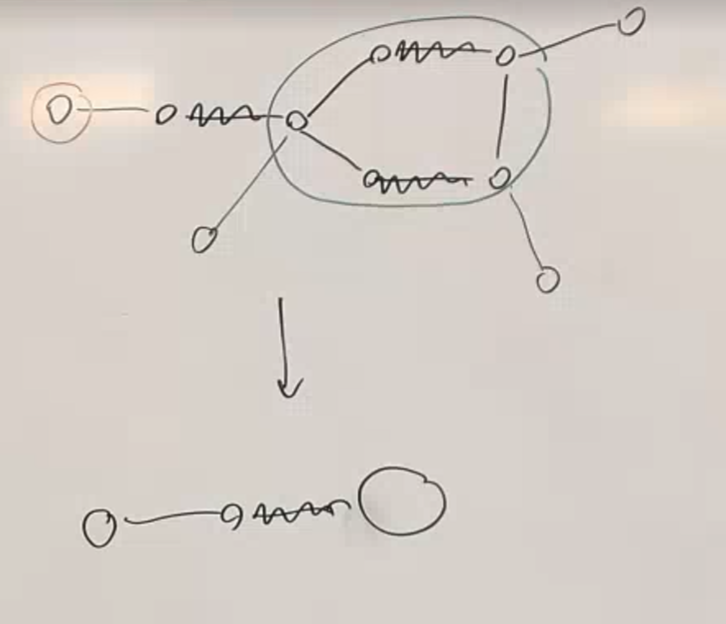
\includegraphics[scale=0.5]{img/parsoch_blossom_cut}
\end{center}

Утверждение: если в исходном графе $G$ был дополняющий путь, то и в полученном графе $G^\prime$.

\begin{proof}
    Докажем в две стороны

    ($\Leftarrow$) Либо дополняющий путь вообще не проходит через большую вершину соцветия, тогда вообще все просто, ничего точно не поломается.\\
    Если дополгяющий путь проходит через большую вершину соцветия, то выберем кусок цикла нужной четности и соееденим кусочки дополняющего пути.
    \begin{center}
        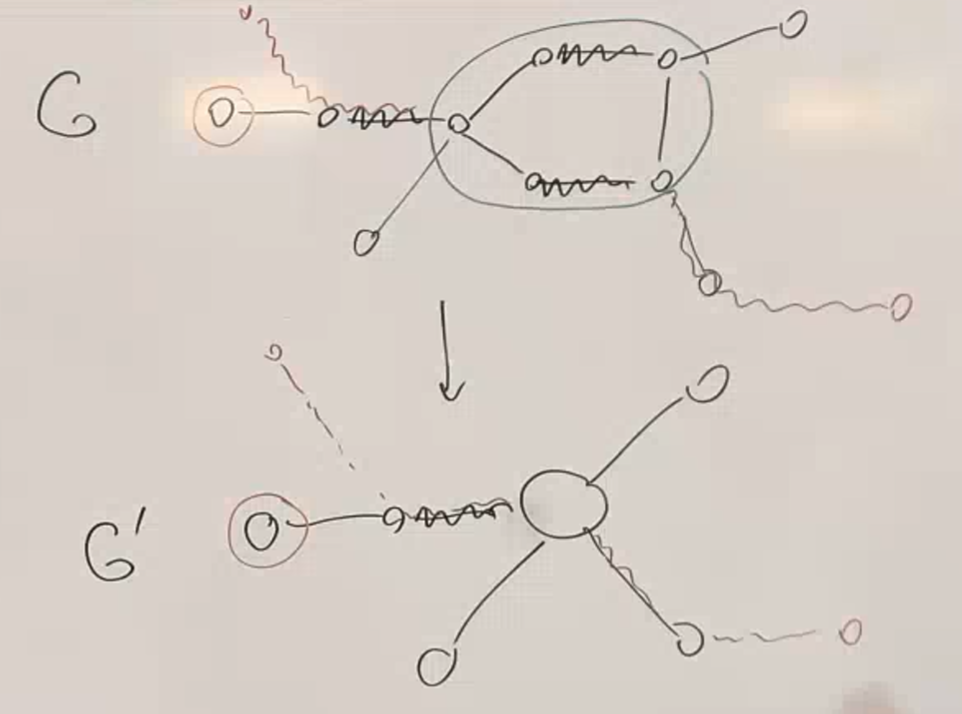
\includegraphics[scale=0.35]{img/parsoch_blossom_cut_proof_1}
    \end{center}

    ($\Rightarrow$) Все сложно.
    Могут быть всякие сложные пути и после сжатия не понятно, что с ними делать.
    Конструктивно доказать сложно.

    Докажем при помощи теоремы о дополняющем пути.
    От противного.
    \begin{enumerate}
        \item Возьмем граф $G$ вместе с соцветием и инвертируем ему стебель,
        получим граф $H$ с валидным парсочем.
        \item Возьмем граф $H$ вместе с соцветием и инвертируем ему стебель,
        получим граф $H^\prime$ с валидным парсочем.

        \item
        Если в $G$ есть дополняющий путь, то и в $G^\prime$ тоже есть дополняющий путь (очевидно, так как и то и другое паросочетание не максимального размера).

        Если в $H^\prime$ есть дополняющий путь, то и в $H$ тоже есть дополняющий путь (очевидно, так как и то и другое паросочетание не максимального размера).

        Если в $G^\prime$ есть дополняющий путь, то и в $H^\prime$ есть дополняющий путь (конструктивно).
        \begin{center}
            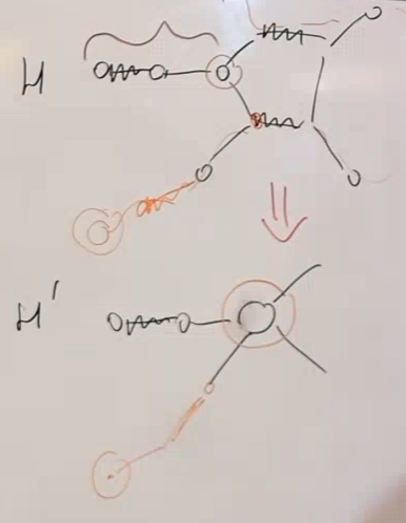
\includegraphics[scale=0.475]{img/parsoch_blossom_cut_proof_2}
        \end{center}
    \end{enumerate}
\end{proof}

\subsubsection*{Алгоритм}

\begin{lstlisting}[mathescape=true]
    M = $\varnothing$
    while True:
        dfs
        if нашли доп путь:
            разжать соцветие
            M++
            continue
        if нет додоп пути, не соцветий:
            break
        if соцветие:
            сжать соцветие
\end{lstlisting}

Итого, время работы алгоритма~--- $\mathcal{O}(n^2 m)$.

Как реализовать побыстрее? \textit{Немного пострадать}.

Пооптимизируем $DFS$.
Прямо проходя в DFS--е можно сжимать вершины.
Для этого можно быстро мерджить списки ребер.

\begin{center}
    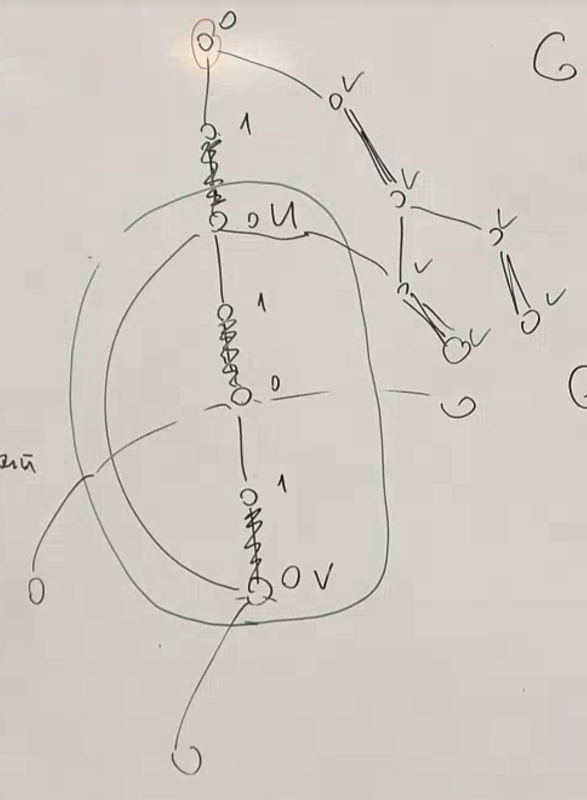
\includegraphics[scale=0.5]{img/parsoch_blossom_cut_fast_dfs}
\end{center}

В общем, если постараться, можно получить решение $\mathcal{O}(n m \alpha (m, n))$.
А вообще, пацаны умеет делать за $\mathcal{O}(m \sqrt{n})$.

\endinput
\end{document}